\documentclass[a4paper, 12pt]{article}

%%% Работа с русским языком
\usepackage{cmap}					% поиск в PDF
\usepackage{mathtext} 				% русские буквы в формулах
\usepackage[T2A]{fontenc}			% кодировка
\usepackage[utf8]{inputenc}			% кодировка исходного текста
\usepackage[russian]{babel}	% локализация и переносы

%%% Дополнительная работа с математикой
\usepackage{amsmath,amsfonts,amssymb,amsthm,mathtools} % AMS
\usepackage{icomma} % "Умная" запятая: $0,2$ --- число, $0, 2$ --- перечисление

%% Номера формул
%\mathtoolsset{showonlyrefs=true} % Показывать номера только у тех формул, на которые есть \eqref{} в тексте.

%% Шрифты
\usepackage{euscript}	 % Шрифт Евклид
\usepackage{mathrsfs} % Красивый матшрифт

%% Поля
\usepackage[left=2cm,right=2cm,top=2cm,bottom=2cm,bindingoffset=0cm]{geometry}

%% Русские списки
\usepackage{enumitem}
\makeatletter
\AddEnumerateCounter{\asbuk}{\russian@alph}{щ}
\makeatother

%%% Работа с картинками
\usepackage{graphicx}  % Для вставки рисунков
\graphicspath{{images/}{images2/}}  % папки с картинками
\setlength\fboxsep{3pt} % Отступ рамки \fbox{} от рисунка
\setlength\fboxrule{1pt} % Толщина линий рамки \fbox{}
\usepackage{wrapfig} % Обтекание рисунков и таблиц текстом

%%% Работа с таблицами
\usepackage{array,tabularx,tabulary,booktabs} % Дополнительная работа с таблицами
\usepackage{longtable}  % Длинные таблицы
\usepackage{multirow} % Слияние строк в таблице

%% Красная строка
\setlength{\parindent}{2em}

%% Интервалы
\linespread{1}
\usepackage{multirow}

%% TikZ
\usepackage{tikz}
\usetikzlibrary{graphs,graphs.standard}

%% Верхний колонтитул
\usepackage{fancyhdr}
\pagestyle{fancy}

%% Перенос знаков в формулах (по Львовскому)
\newcommand*{\hm}[1]{#1\nobreak\discretionary{}
	{\hbox{$\mathsurround=0pt #1$}}{}}

%% Мои дополнения
\usepackage{float} %Добавляет возможность работы с командой [H] которая улучшает расположение на странице
\usepackage{gensymb} %Красивые градусы
\usepackage{graphicx}               % Импорт изображений
\usepackage{caption} % Пакет для подписей к рисункам, в частности, для работы caption*
\usepackage{indentfirst}


\begin{document}

\newcommand{\HRule}{\rule{\linewidth}{0.7mm}} % Defines a new command for the horizontal lines, change thickness here
	
	\begin{center}
		\large\textbf{Московский Физико-Технический Институт}\\ % Name of your university/college
		\large\textbf{(государственный университет)}
	
		\vfill
		
		\Large Лабораторная работа по курсу общей физики № 4.5.3\\[0.5cm] % Preambule of your document title
		
		
		\HRule
		\\[0.4cm]
		{ \huge \bfseries Сканирующий интерферометр}% Title of your document
		\\[0.4cm] 
		\HRule
		\\[0.5cm]
		
		\ \\
	\textbf{\large Автор:} \\	
	\large Лепарский Роман Б01-003\\ % Your name and something more, your group num for example
		\vfill
		\hspace*{-0.8 cm}
\includegraphics[width=100 pt]{frkt_logo}\\ % logo of your  company/university/college
		\large Долгопрудный, 2022 % location and year
	\end{center}

\newpage
\setcounter{page}{2}
\fancyfoot[c]{\thepage}
\fancyhead[L] {Работа № 4.5.3} % some information in page header
\fancyhead[R]{}

\section{Аннотация}

\textbf{Цель работы}: определение дифракционного предела разрешения объектива микроскопа.

\textbf{В работе используются}: лазер; кассета с набором сеток разного периода; щель с микрометрическим винтом; оптический стол с набором рейтеров и крепёжных винтов; экран; линейка.


\section{Теоретические сведения}
Для иммерсионного микроскопа разрешающая способность объектива при некогерентном освещении
\begin{equation}
\ell_{min} \approx \dfrac{0.61\lambda}{\sin u},
\end{equation}
где $u$ -- апертурный угол объектива микроскопа (угол между оптической осью и лучом, направленным из центра объекта в край линзы).

Метод Аббе для оценки разрешающей способности состоит в разделении хода лучей на две части: сначала рассматривается картина в задней фокальной плоскости $F$ объектива -- она называется первичным изображением. Это первичное изображение рассматривается как источник волн, создающий вторичное изображение в плоскости $P_2$, сопряжённой плоскости предмета.\\
Первичное изображение есть картина дифракции Фраунгофера (на дифракционной решётке), если её период $d$, то для направления максимальной интенсивности $\varphi_m$
\begin{equation}
d \sin \varphi_m = m\lambda.
\end{equation}
При этом проходят пучки только с $\varphi_m < u$. Можно условием разрешения считать, что $u > \varphi_1$, иначе говоря
$$
\sin u \geq \lambda/d.
$$
или
\begin{equation}
\label{equ:allow}
d \geq \dfrac{\lambda}{\sin u} \approx \dfrac{\lambda}{D/2f},
\end{equation}
где $D$ -- диаметр линзы, $f$ -- фокусное расстояние.\\
Сетку можно рассматривать как две перпендикулярные друг другу решетки, для максимумов которых выполняется соотношение
\begin{equation}
\begin{array}{c c}
d\sin \varphi_x = m_x \lambda, & d\sin \varphi_y = m_y \lambda. \\
\end{array}
\end{equation}
\newpage
\section{Экспериментальная установка}
\begin{figure}[h]
	\centering
	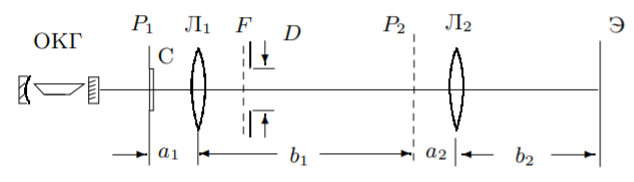
\includegraphics[scale=0.7]{stand.png}
	\caption{Схема установки}
	\label{fig:stand}
\end{figure}
Схема установки приведена на Рис. \ref{fig:stand}. Предметом $P_1$ служат сетки в кассете $C$. Линза $\text{Л}_1$ длиннофокусная, а $\text{Л}_2$ короткофокусная. В $F$ устанавливаются диафрагмы $D$, с помощью сеток с разными $d$ и щелевой диафрагмы можно проверить соотношение (\ref{equ:allow}). Период сеток может быть измерен либо по расстоянию между дифракционными максимумами на экране, либо по увеличенному с помощью микроскопа изображению. Пространственную фильтрацию (получение наклонного изображение решётки) можно получить с помощью подбора угла наклона и ширины вспомогательной щели.

\section{Обработка результатов}

	Запишем данные лабораторной установки:
	\begin{table}[H]
		\centering
		\begin{tabular}{|l|l|l|}
			\hline
			$\lambda$, нм & $f_1$, мм & $f_2$, мм \\ \hline
			532           & 110       & 25        \\ \hline
		\end{tabular}
	\end{table}

	\subsection{Определение периода решеток по их пространственному спектру}
	Расстояние от дифракционной решетки до экрана $H = 1257 \pm 3$ мм. Погрешность учитывает невозможность определить точное положение решетки в кассете. Для каждой сетки определим расстояние между максимумами $l$, их количество $n$ и посчитаем период сетки $d$. Погрешность измерения расстояния обусловлена невозможностью достоверно определить центр пятна. Так же, для последней решетки тяжело точно посчитать количество максимумов.
	
	\begin{table}[H]
		\centering
		\begin{tabular}{|l|l|l|l|}
			\hline
			$N$ & $l$, мм    & $n$       & $d$, нм \\ \hline
			1   & 202$\pm 2$ & 6         & 20000   \\ \hline
			2   & 247$\pm 2$ & 11        & 30000   \\ \hline
			3   & 269$\pm 2$ & 24        & 61000   \\ \hline
			4   & 274$\pm 1$ & 49        & 122000  \\ \hline
			5   & 276$\pm 1$ & 66$\pm 1$ & 163000  \\ \hline
		\end{tabular}
	\end{table}

	Максимальная погрешность периода решетки по формуле косвенных измерений $\sigma_d \hm= 1$ мкм.
	
	\subsection{Определение периода решеток по изображению, увеличенному с помощью микроскопа}
	
	Запишем параметры настроенного микроскопа.
	\begin{table}[H]
		\centering
		\begin{tabular}{|l|l|l|}
			\hline
			$a_1$, мм  & $b_1+a_2$, мм & $b_2$, мм  \\ \hline
			$115\pm 5$ & $562\pm 5$    & $424\pm 5$ \\ \hline
		\end{tabular}
	\end{table}
	Погрешность обусловлена невозможностью точно определить центр линзы. Приняв $a_2 = f_2$ найдем $b_1 = 380 \pm5$ мм. Увеличение получившейся системы:
	\[
		\Gamma = \frac{b_1b_2}{a_1a_2} = 79 \pm 5
	\]
	Запишем количество периодов сетки и расстояние между ними, а так же посчитаем период по формуле $d = l/(n\Gamma)$
	\begin{table}[H]
		\centering
		\begin{tabular}{|l|l|l|l|l|}
			\hline
			$N$ & $l$, мм & $n$ & $d$, нм & $\sigma_d$, нм \\ \hline
			1   & 112     & 67  & 21000   & 1480       \\ \hline
			2   & 157     & 65  & 30000   & 1991       \\ \hline
			3   & 160     & 33  & 61000   & 3884       \\ \hline
			4   & 205     & 21  & 123000  & 7820       \\ \hline
			5   & 203     & 15  & 170000  & 10842      \\ \hline
		\end{tabular}
	\end{table}
	Видно, что значения совпадают в пределах погрешности.
	
	\subsection{Определение периодов решеток по оценке разрешающей способности микроскопа}
	
	Если поместить в фокальную плоскость линзы Л$_1$ щелевую диафрагму, то при минимальном раскрытии, при котором будет видна решетка, ее период будет определяться так
	\[
		d = \frac{2\lambda f_1}{D}
	\]
	Примем погрешность измерения $\sigma_D = 0,02$ мм.
	Запишем результаты в таблицу
	\begin{table}[H]
		\centering
		\begin{tabular}{|l|l|l|l|}
			\hline
			$N$ & $D$, мм & $d$, нм & $\sigma_d$ \\ \hline
			2   & 4,2     & 27800   & 132        \\ \hline
			3   & 1,92    & 60900   & 634        \\ \hline
			4   & 0,93    & 125000  & 2706       \\ \hline
			5   & 0,66    & 177000  & 5373       \\ \hline
		\end{tabular}
	\end{table}
	Видно, что результаты совпадают с предыдущими экспериментами.
	
	Теперь проверим справедливость этой формулы построив график $d = f(1/D)$
	\begin{figure}[H]
		\centering
		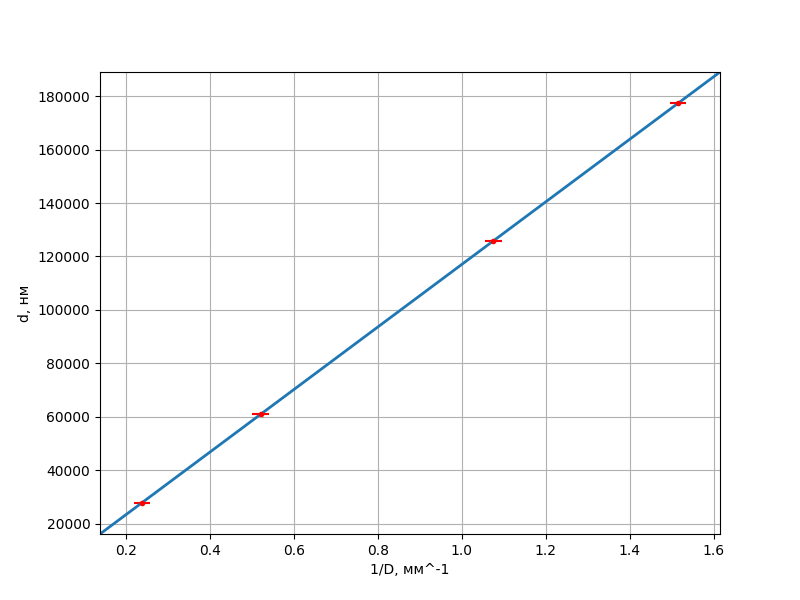
\includegraphics[scale = 0.7]{abbe.png}
	\end{figure}

	Данные хорошо аппроксимируются прямой, поэтому можно говорить о справедливости этой формулы.
	
	\section{Вывод}
	В этой работе мы познакомились с устройством и принципом действия микроскопа, а так же нашли периоды дифракционных решеток 3 способами. Данные соответствуют друг другу в каждом эксперименте.















\end{document}